\documentclass[a4paper, 10pt]{article}    
\usepackage{geometry}       
\geometry{a4paper}
\geometry{margin=1in} 
\usepackage{paralist}
  \let\itemize\compactitem
  \let\enditemize\endcompactitem
  \let\enumerate\compactenum
  \let\endenumerate\endcompactenum
  \let\description\compactdesc
  \let\enddescription\endcompactdesc
  \pltopsep=\medskipamount
  \plitemsep=1pt
  \plparsep=1pt
\usepackage[english]{babel}
\usepackage[utf8]{inputenc}

\usepackage{bbm, bm}
\usepackage{amsmath, amssymb, amsthm, mathrsfs}
\usepackage{booktabs, tikz}

\pagestyle{headings}
\newcommand{\boxwidth}{430pt}

\theoremstyle{definition}
\newtheorem{problem}{Problem}

\newtheoremstyle{hSol}
  {1.0pt}% Space above
  {1.0pt}% Space below
  {}% bodyfont
  {}% indent
  {\bfseries}% thm head font
  {.}% punctuation after thm head
  { }% Space after thm head
  {}% thm head spec

\theoremstyle{hSol}
\newtheorem*{solution}{Solution}



\title{\textbf{Numerical Solutions for DEs HW2}}
\author{YANG, Ze (5131209043)}


\begin{document}
\maketitle


%------------------------------------------------------------------------
~\\
\fbox{
  \parbox{\boxwidth}{
  \textbf{A Note to TA}: 
  ~\\
  \emph{Hi, this is the senior student from Antai College who did not register for this course. I would like to do all the assignments for practice, but feel free to just skip my homework if you don't have time.
  Thank you again for allowing me to access the assignments and other class material! : )}
  ~\\
  \emph{- Ze}
  }
}

~\\
~\\
%------------------------------------------------------------------------

\begin{problem}
\begin{itemize}
  \item[a.] Implement \emph{RK2}, \emph{Heun's Method} and the classical \emph{RK4}, and justify the rate of convergence numerically.
  \item[b.] Choose appropriate Runge-Kutta method to initialize \emph{Adams-Bashforth} method of order 3,
  $$
  y_{n+3} = y_{n+2} + h [\tfrac{23}{12}f(t_{n+2}, y_{n+2}) - \tfrac{4}{3} f(t_{n+1}, y_{n+1}) + \tfrac{5}{12}f(t_n, y_n)]
  $$
  Justify the rate of convergence numerically.
\end{itemize}
\end{problem}
\begin{solution} We solve the test case 6: $y'=t^2 - y$ with all the five methods above.

\begin{center}
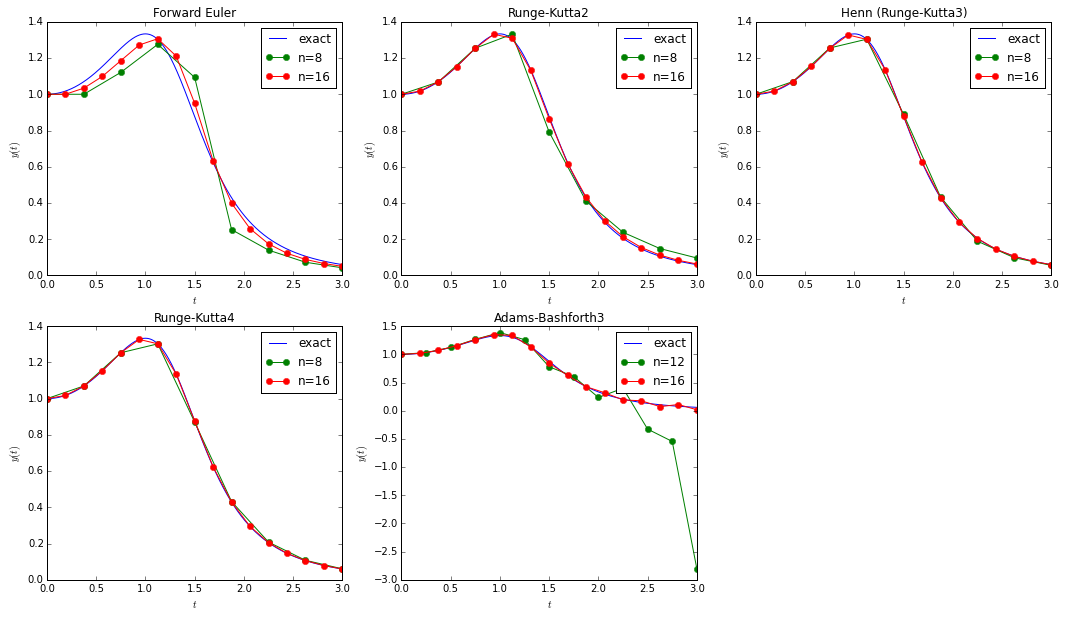
\includegraphics[scale=0.4]{hw2_p1.png}
\end{center}
Where the \emph{Adams-Bashforth} multistep method is intialized with a 3-order method (Heun's method). 

~\\
We plot $\log(n)$ against $\log(error)$ to check the rate of convergence. Theoretically, for a method of order $k$, we expect to get a line with slope $-k$.

\begin{center}
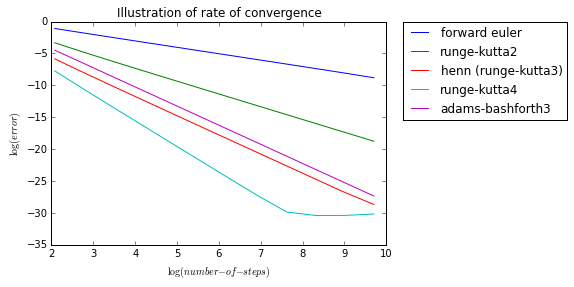
\includegraphics[scale=0.7]{hw2_p2.png}
\end{center}

~\\
From the figure above we know that it is indeed the case. The curve for 4-th order Runge-Kutta method becomes flat in the end because the round-off error will dominate the error of the algorithm for $n$ sufficiently large. And from the figure we know that the round-off error may be $\sim 2^{-30}$.

~\\
We also investigate the running time. The slope of these curves are 1, because all the algorithms take $O(n)$ time, regardless of their orders.

\begin{center}
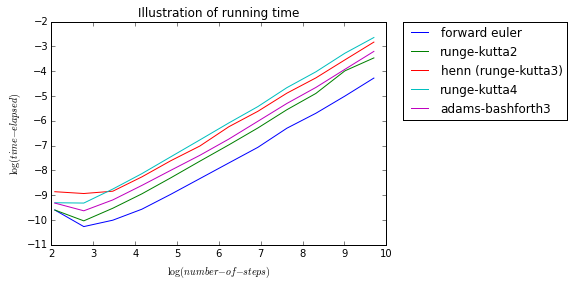
\includegraphics[scale=0.7]{hw2_p3.png}
\end{center}


Please also see the attached code for details.
\end{solution} 
\noindent\rule{16cm}{0.4pt}
%///////////////////////////////////////////////////////////////////////

\begin{problem} Consider the RK method (I just use the notations in the class)
$$
\frac{y_{n+1}-y_n}{h} = c_1k_1 + c_2 k_2
$$
where $k_1= f(t_n, y_n), k_2 = f(t_n+b_{21}h, y_n + b_{21}h k_1)$, and $c_1, c_2, b_{21} \in \mathbb{R}$. 
\begin{itemize}
  \item[a.] Show that there is a choice of these parameters such that the truncation error of the method
  $$
  \frac{T_n}{\Delta t} = \frac{y(t_{n+1})-y(t_n)}{h} - c_1f(t_n, y(t_n)) - c_2 f(t_n+b_{21}h, y(t_n) + b_{21}h f(t_n, y(t_n)))
  $$
  is of order 2 as $h \to 0$.
  \item[b.] Suppose that a second order method of the above form is applied to the IVP $y'=-\lambda y$, $y(0)=1$, where $\lambda$ is \emph{real positive} number. Show that the sequence $\{y_n\}_{n\geq 0}$ is bounded $\iff$ $h \leq 2/\lambda$ (like the interval of absolute stability). Show further that, for such $\lambda$: $|y(t_n) - y_n|\leq \frac{1}{6}\lambda^3 h^2 t_n$, $n\geq 0$.
\end{itemize}
\end{problem}
\begin{proof} (a) We have (by $f$ we mean $f(t_n, y(t_n))$, and by $y$ we mean $y(t_n)$):
\begin{equation}
  \begin{split}
    y'&=f \\
    y'' &= f_t + f_yy' = f_t + f_y f\\
    y'''&=f_{tt} + f_{ty} y' + y''f_y + (f_y)'y' = f_{tt}+2f_{ty}f+f^2 f_{yy}+f_y f_t + f_y^2 f
  \end{split}
\end{equation}
Therefore use taylor expansion of $y(t_{n+1})$ at $t_n$: 
\begin{equation}
  \frac{y(t_{n+1}) - y(t_n)}{h} = f + \frac{h}{2}(f_t + f_y f) + \frac{h^2}{6}(f_{tt}+2f_{ty}f+f^2 f_{yy}+f_y f_t + f_y^2 f)  
\end{equation}
And that
\begin{equation}
  \begin{split}
    b_1 k_1 + b_2 k_2 &= b_1 f + b_2 f(t_n + c_2 h, y(t_n) + ha_{21}f(t_n, y(t_n))) \\
    &= b_1 f + b_2 (f + f_t c_2 h + f_y ha_{21}f + \tfrac{1}{2}(f_{tt}c_2^2h^2+2f_{ty} c_2 h \cdot a_{21}hf + f_{yy}h^2 a_{21}^2 f^2+O(h^3)) \\
    &= (b_1 + b_2)f + h(b_2 c_2 f_t + b_2 a_{21}f_yf) + \tfrac{h^2}{2}(c_2^2 f_{tt}+2c_2a_{21}f_{ty}f+a_{21}f_{yy}f^2) + O(h^3)
  \end{split}
\end{equation}
So we subtract $b_1 k_1 + b_2 k_2$ from $\frac{y(t_{n+1})-y(t_n)}{h}$. To achieve a truncation error of order $2$, we have to let $O(1)$ and $O(h)$ terms equal to 0:
\begin{equation}
  \begin{split}
    O(1)\text{ terms}: & f  - (b_1 + b_2)f = 0 \\
    O(h)\text{ terms}: & \frac{h}{2}(f_t + f_y f)  - h(b_2 c_2 f_t + b_2 a_{21}f_yf) = 0 \\
  \end{split}
\end{equation}
$$
  \Rightarrow b_1 + b_2 = 1;~~~b_2 c_2 = \tfrac{1}{2};~~~b_2 a_{21}=\tfrac{1}{2}
$$
Clearly, there exists such parameters. For example, $b_1 = b_2 = \frac{1}{2}$, $a_{21}=c_2=1$. $\square$

~\\
(b.) Apply RK2 to $y'=- \lambda y$: $k_1 = - \lambda y_n$. $k_2 = -\lambda (y_n + a_{21} hk_1)$. So let $z := \lambda h$
$$
y_{n+1} = y_n + h (-b_1 \lambda y_n - b_2 \lambda y_n + b_2 a_{21} h \lambda^2 y_n) = y_n (1-b_1 z-b_2z + b_2 a_{21} z^2) = y_n(1-z+\tfrac{1}{2}z^2)
$$
Therefore $y_n = (1-z+\tfrac{1}{2}z^2)^n y_0$ is bounded $\Rightarrow |1-z+\tfrac{1}{2}z^2|\leq 1$. The solution is $0\leq z\leq 2$, i.e. $h\leq 2/\lambda$. \\
The exact solution $y(t_n) = e^{-\lambda t}y(0) = e^{-nz}$. Hence 
$$
y(t_n) - y_n = e^{-nz} - (1-z+\tfrac{1}{2}z^2)^n
$$
Use taylor expansion to $e^{-nz}$, and trinomial expansion to the second term:
$$
e^{-nz} = 1 - nz + \frac{n^2 z^2}{2} - \frac{n^3z^3}{6} + \frac{n^4z^4}{24} + h.o.t.
$$
\begin{equation}
  \begin{split}
    (1-z+\tfrac{1}{2}z^2)^n &= 1 + n(-z) + n(\tfrac{z^2}{2}) + \tfrac{n(n-1)}{2!}(-z)^2 + \tfrac{n(n-1)}{1!1!}(-z)(\tfrac{z^2}{2}) + \tfrac{n(n-1)(n-2)}{3!}(-z)^3 \\
    &~~~~+ \tfrac{n(n-1)(n-2)(n-3)}{4!}(-z)^4 + \tfrac{n(n-1)}{2!}(\tfrac{z^2}{2})^2 + \tfrac{n(n-1)(n-2)}{2!1!}(-z)^2(\tfrac{z^2}{2})+h.o.t. \\
    &= 1-nz + \tfrac{(n^2-n+n)}{2} z^2- \tfrac{[(n^3-3n^2+2n)+(3n^2-3n)]}{6}z^3\\
    &~~~~+\tfrac{[(n^4-6n^3+11n^2-6n)+(3n^2-3n)+(6n^3-18n^2+12n)]}{24}z^4 + h.o.t\\
    &=1-nz + \tfrac{n^2}{2}z^2 - \tfrac{n^3-n}{6}z^3 + \tfrac{n^4-4n^2+3n}{24}z^4  + h.o.t.
  \end{split}
\end{equation}
Hence
\begin{equation}
  \begin{split}
    y(t_n) - y_n &= -\frac{n}{6}z^3 + \frac{4n^2-3n}{24}z^4 + h.o.t. \\
    &= -\frac{1}{6}\lambda^3 h^2 t_n + \frac{4n^2-3n}{24}z^4 + h.o.t.
  \end{split}
\end{equation}
For $n \in \mathbb{N}^{+} \cup \{0\}$, we have $4n^2-3n \geq 0$. Therefore
$$
|y(t_n) - y_n| = \left|-\frac{1}{6}\lambda^3 h^2 t_n + \frac{4n^2-3n}{24}z^4 + h.o.t.\right| \leq \left|\frac{1}{6}\lambda^3 h^2 t_n\right|
$$
As $h\to 0$, $z=\lambda h\to 0$.

\end{proof} 
\noindent\rule{16cm}{0.4pt}
%///////////////////////////////////////////////////////////////////////

\begin{problem} Find the general solution $\{y_n\}$ for the homogeneous recurrence reltation
$$
a_0 y_n + a_1 y_{n+1} + ... + a_s y_{n+s} = 0
$$
\end{problem}
\begin{proof} WLOG we assume the recurrence is of order $s$, i.e. $a_s \ne 0$. Then rearrange the terms as:
$$
y_{n+s} + \tfrac{a_{s-1}}{a_s} y_{n+s-1} + ... + \tfrac{a_{1}}{a_s} y_{n+1} + \tfrac{a_{0}}{a_s} y_{n+1} = y_{n+s} + c_{s-1}y_{n+s-1} + ... + c_1 y_{n+1} + c_0 y_{n} = 0
$$
with $c_k=\frac{a_k}{a_s}$, $k=0,1,...,s-1$.
We start with a lemma on \emph{companion matrix}.
\begin{itemize}
  \item[\textit{Lemma.}] The chracteristic polynomial of $n$-degree $P(\lambda)=\lambda^s + c_{s-1}\lambda^{s-1}+...+c_1 \lambda + c_0 = \det(\lambda \bm{I} - \bm{C})$, where 
  $$
  \bm{C} = \begin{pmatrix}
    -c_{s-1} & -c_{s-2} & \hdots & -c_1 & -c_0 \\
    1 & 0 & \hdots & 0 & 0\\
    0 & 1 & \hdots & 0 & 0\\
    \vdots & \vdots & \ddots & \vdots & \vdots\\
    0 & 0 & \hdots & 1 & 0\\
  \end{pmatrix}
  $$
\end{itemize}
\emph{Proof of Lemma}: We prove by induction. For degree $s=1$ case, $P(\lambda) = \lambda + c_0$. And $\lambda \bm{I} - \bm{C}$ is just $\lambda - (-c_0)$. \\
Now assume the relation is true for $s-1$, at $s$, we have $\det(\lambda\bm{I} - \bm{C}) = $
$$
\begin{vmatrix}
    c_{s-1} & c_{s-2} & \hdots & c_1 & c_0 \\
    -1 & \lambda & \hdots & 0 & 0\\
    0 & -1 & \hdots & 0 & 0\\
    \vdots & \vdots & \ddots & \vdots & \vdots\\
    0 & 0 & \hdots & -1 & \lambda\\
\end{vmatrix}_{s} = \lambda \begin{vmatrix}
    c_{s-1} & c_{s-2} & \hdots & c_2 & c_1 \\
    -1 & \lambda & \hdots & 0 & 0\\
    0 & -1 & \hdots & 0 & 0\\
    \vdots & \vdots & \ddots & \vdots & \vdots\\
    0 & 0 & \hdots & -1 & \lambda\\
\end{vmatrix}_{s-1} + (-1)^{s+1} c_0 
\begin{vmatrix}
    -1 & \lambda & \hdots & 0 & 0\\
    0 & -1 & \hdots & 0 & 0\\
    \vdots & \vdots & \ddots & \vdots & \vdots\\
    0 & 0 & \hdots & -1 & \lambda\\
    0 & 0 & \hdots & 0 & -1\\
\end{vmatrix}_{s-1}~~(\dag)
$$
with our inductive assumption, the determinant in the first term is exactly $\det (\lambda \bm{I} - \bm{C})$ in the degree $s-1$ case. So,
$$
(\dag) = \lambda (\lambda^{s-1}+c_{s-1} \lambda^{s-2} + ... + c_2 \lambda + c_1) + (-1)^{s+1} c_0 (-1)^{s-1} = P(\lambda)~~~~\blacksquare
$$
The lemma suggests that finding the roots of $P(\lambda)=0$ is equivalent to finding the eigenvalues of $\bm{C}$. \\
We denote $\bm{y}_n = (y_{n+s}, ..., y_{n+2}, y_{n+1})^{\top}$; $\bm{c}=(c_{s-1}, ..., c_1, c_0)^{\top}$, and unit vector with 1 on position $k$ as $\bm{\iota}_k$. We find that the linear recurrence can be vectorized as $y_{n+s} = -\bm{c}^{\top} \bm{y}_{n-1}$. Moreover $y_{n+k} = \bm{\iota}_k^{\top} \bm{y}_{n-1}$ for $k=1, ..., s-1$.
$$
\bm{y}_{n} = \begin{pmatrix}
  y_{n+s} \\
  y_{n+s-1} \\
  y_{n+s-2} \\
  \vdots \\
  y_{n+1}
\end{pmatrix} = 
\begin{pmatrix}
  -\bm{c}^{\top}\bm{y}_n \\
  \bm{\iota}_{1}^{\top}\bm{y}_n \\
  \bm{\iota}_{2}^{\top}\bm{y}_n \\
  \vdots \\
  \bm{\iota}_{s-1}^{\top}\bm{y}_n
\end{pmatrix}
= 
\begin{pmatrix}
    -c_{s-1} & -c_{s-2} & \hdots & -c_1 & -c_0 \\
    1 & 0 & \hdots & 0 & 0\\
    0 & 1 & \hdots & 0 & 0\\
    \vdots & \vdots & \ddots & \vdots & \vdots\\
    0 & 0 & \hdots & 1 & 0\\
\end{pmatrix} 
\begin{pmatrix}
  y_{n+s-1} \\
  y_{n+s-2} \\
  y_{n+s-3} \\
  \vdots \\
  y_{n}
\end{pmatrix} = \bm{Cy}_{n-1} = \bm{C}^{n} \bm{y}_0
$$
where $\bm{y}_0 = (y_s, y_{s-1}, ..., y_2, y_1)^{\top}$ is the initial condition.\\
Assume $\bm{C}$ has eigenvalues $\lambda_1, ..., \lambda_p$, $p\leq s$ with algebraic multiplicity $m_1, ..., m_p$, where $\sum_p m_p = s$. Hence we decompose $\bm{C} = \bm{PJ}\bm{P}^{-1}$ in its Jordan Normal Form: 
$$
\bm{C}^n \bm{y}_0 = \bm{P} \bm{J}^n \bm{P}^{-1} \bm{y}_0 = \bm{P} \begin{pmatrix}
  \bm{J}_{\lambda_1}^n & & \\
  & \bm{J}_{\lambda_2}^n &  \\
  & & \ddots & \\
  & & & \bm{J}_{\lambda_p}^n
  \\
\end{pmatrix} \bm{P}^{-1} \bm{y}_0~~(*)
$$
$$
\text{where } \bm{J}_{\lambda_i}^n = 
\begin{pmatrix}
   \lambda_i^n & \binom{n}{1} \lambda_i^{n-1} & \binom{n}{2} \lambda_i^{n-2} & \hdots & \binom{n}{m_{i}-1} \lambda_i^{n-(m_i-1)}\\
   & \lambda_i^n & \binom{n}{1} \lambda_i^{n-1} & \hdots & \binom{n}{m_{i}-2} \lambda_i^{n-(m_i-2)}\\
   & & \ddots & \ddots & \vdots \\
   & & & \lambda_i^n &  \binom{n}{1} \lambda_i^{n-1}\\
   & & & & \lambda_i^n
\end{pmatrix}_{m_i \times m_i}
$$
The typical entry is $\binom{n}{r} \lambda_i^{n-r} = \frac{\binom{n}{r}}{\lambda_i^r} \lambda_i^n$, which we can regard as $p^{[r]}_i(n) \lambda_i^n$. Here $p^{[r]}_i(n)$ is a polynomial of $n$ to the degree $r$. Therefore, we regard $(*)$ as applying linear opeartions on these entries. We know that applying linear operations on a collection of polynomials $\{p^{[r]}_i(n)\}_{r=1}^{m_i-1}$ will result in another polynomial with degree no more than $m_i-1$, denote it as $g_i^{[m_i-1]}(n)$. So we have
\begin{equation}
  \begin{split}
    y_{n+s} &= \sum_{i=1}^p g^{[m_i-1]}_i(n) \lambda_i^n = \sum_{i=1}^p  \sum_{r=0}^{m_i-1} \alpha_{ir} n^r \lambda_i^n \\
    &= (\alpha_{10} + \alpha_{11}n + ... + \alpha_{1,m_1-1} n^{m_1-1}) \lambda_1^n + ... + (\alpha_{p0} + \alpha_{p1}n + ... + \alpha_{p,m_p-1} n^{m_p-1}) \lambda_p^n
  \end{split}
\end{equation}
Where $\{\alpha_{ir}\}_{i=1, r=0}^{p, m_i-1}$ are constants. Since $\sum_{i=1}^p m_i = s$, there are $s$ constants in total, which are solved by inserting initial condition $\bm{y}_0=(y_s, y_{s-1}, ..., y_1)^{\top}$ into the general solution. If we index the initial condition as $(y_0, y_{-1}, ..., y_{-(s-1)})^{\top}$ instead, the general solution will be
$$
y_{n} = (C_{10} + C_{11}n + ... + C_{1,m_1-1} n^{m_1-1}) \lambda_1^n + ... + (C_{p0} + C_{p1}n + ... + C_{p,m_p-1} n^{m_p-1}) \lambda_p^n
$$
Where $\{C_{ir}\}$ is another set of constants. By lemma, $\{\lambda_i\}$ are the roots of $P(\lambda)=0$, with multiplicity $\{m_i\}$. And this general solution holds for all $n\geq 0$.

\end{proof}
\noindent\rule{16cm}{0.4pt}
%///////////////////////////////////////////////////////////////////////

\begin{problem} Find the region of A-stablity for the multistep method:
$$
y_{n+2} - y_n = \frac{1}{3}h [f(t_{n+2}, y_{n+2}) + 4f(t_{n+1}, y_{n+1}) + f(t_n, y_n) ]
$$
\end{problem}
\begin{proof} The first- and second-characteristic polynomial of the method is:
$$
\rho(z) = z^2 - z;~~~\sigma(z) = \tfrac{1}{3}z^2+\tfrac{4}{3}z+\tfrac{1}{3}
$$
So the method is absolute stable $\iff$ the roots $z$ of $\Pi(z,\bar{h})=\rho(z)-\bar{h}\sigma(z)$ have modulus $<1$.
\begin{equation}
  \Pi(z,\bar{h}) = z^2 - z - \bar{h}\left(\tfrac{1}{3}z^2+\tfrac{4}{3}z+\tfrac{1}{3}\right) = (1-\tfrac{\bar{h}}{3})z^2 + (-1-\tfrac{4\bar{h}}{3})z + (-\tfrac{\bar{h}}{3}) = 0
\end{equation}
We solve the equation and obtain
$$
z = \frac{\pm\sqrt{3(4 \bar{h}^2+12 \bar{h}+3)}-4 \bar{h}-3}{2 (\bar{h}-3)}
$$
Or $\bar{h} = (z^2 - z)/(\tfrac{1}{3}z^2+\tfrac{4}{3}z+\tfrac{1}{3})$. Denote the stability region as $\mathcal{S}$, then on $\partial \mathcal{S}$, the polynomial has root $|z|=1$. Hence we can find the boundary by
$$
\partial \mathcal{S} = \left\{\frac{\rho(e^{i\theta})}{\sigma(e^{i\theta})}, \theta\in [0, 2\pi]\right\} =  \left\{\frac{e^{2i\theta} - e^{i\theta}}{\tfrac{1}{3}e^{2i\theta}+\tfrac{4}{3}e^{i\theta}+\tfrac{1}{3}}, \theta\in [0, 2\pi]\right\}
$$
The region is give as the following plot (please also see the attached code).
\begin{center}
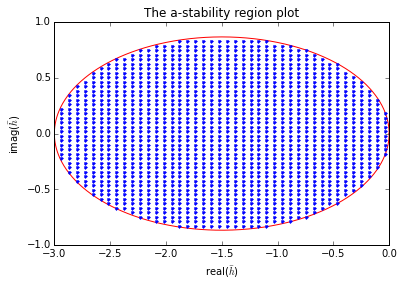
\includegraphics[scale=0.7]{hw2_p4.png}
\end{center}
\end{proof} 
\noindent\rule{16cm}{0.4pt}
%///////////////////////////////////////////////////////////////////////

\begin{problem} (Iserles 3.4) Apply the classical RK4 method (with coefficient table shown as below) to scalar autonomous ode $y'=f(y)$, check that this method is indeed of order 4.
  \begin{center}
    \begin{tabular}{c|ccccc}
    $c_1$ \\
    $c_2$ & $a_{21}$ \\
    $c_3$ & $a_{31}$ & $a_{32}$\\
    $c_4$ & $a_{41}$ & $a_{42}$ & $a_{43}$\\
    \hline
     & $b_1$ & $b_2$ & $b_3$ & $b_4$
    \end{tabular}  = 
    \begin{tabular}{c|ccccc}
    $0$ \\
    $1/2$ & $1/2$ \\
    $1/2$ & $0$ & $1/2$\\
    $1$ & $0$ & $0$ & $1$\\
    \hline
     & $1/6$ & $1/3$ & $1/3$ & $1/6$
    \end{tabular}
  \end{center}
\end{problem}

\begin{proof} We want to calculate the truncation error:
$$
\frac{T_n}{h} = \frac{y(t_{n+1})-y(t_n)}{h} - (b_1k_1 + b_2 k_2 + b_3 k_3 + b_4k_4)
$$
We first calculate the first term using taylor expansion. We calculate the derivatives with \texttt{Mathematica}:
\begin{equation}
  \begin{split}
    y' &= f(y(t)) = f,~~~~\tfrac{1}{2!}y^{(2)} = y'(t) f'(y(t)) = \tfrac{1}{2}f_yf \\
    \tfrac{1}{3!}y^{(3)} &= \tfrac{1}{6}y'(t)^2 f''(y(t))+\tfrac{1}{6}y''(t) f'(y(t)) = \tfrac{1}{6}f_{yy}f^2 + \tfrac{1}{6}f_y^2 f\\
    \tfrac{1}{4!}y^{(4)} &=\tfrac{1}{24}[f^{(3)}(y(t)) y'(t)^3+3 y'(t) y''(t) f''(y(t))+y^{(3)}(t) f'(y(t))]\\
    &= \tfrac{1}{24}[f_{yyy}f^3 + 3f(ff_y)f_{yy} + (f^2f_{yy} + f_y^2 f)f_y] \\
    &= \tfrac{1}{24}f_{yyy}f^3 + \tfrac{1}{6}f_{yy}f_yf^2 + \tfrac{1}{24}f_y^3 f
  \end{split}
\end{equation}
Then we expand the second part, the $k$'s are given by
\begin{equation}
  \begin{split}
    k_1 &= f \\
    k_2 &= f(y_n + \tfrac{1}{2}hf(y_n)) = \{f+f_y\cdot(\tfrac{1}{2}hf) + \tfrac{f_{yy}}{2}\cdot(\tfrac{1}{2}hf))^2+\tfrac{f_{yyy}}{6}\cdot(\tfrac{1}{2}hf)^3+O(h^4)\}\\
    &= f + \tfrac{1}{2}f_yf h + \tfrac{1}{8}f_{yy}f^2 h^2 + \tfrac{1}{48}f_{yyy}f^3 h^3 + O(h^4)
    \end{split}
\end{equation}
\begin{equation}
  \begin{split}
    k_3 &= f\left(y_n + \tfrac{1}{2}h\left(f + \tfrac{1}{2}f_yf h + \tfrac{1}{8}f_{yy}f^2 h^2 + \tfrac{1}{48}f_{yyy}f^3 h^3 + O(h^4)\right)\right)\\
    &= \Big\{
    f + 
    f_y\cdot \tfrac{1}{2}h \left(f + \tfrac{1}{2}f_yf h + \tfrac{1}{8}f_{yy}f^2 h^2 + O(h^3)\right) + 
    \tfrac{f_{yy}}{2}\cdot \tfrac{1}{4}h^2 \left(f + \tfrac{1}{2}f_yf h + O(h^2)\right)^2 + 
    \\
    &~~~~+\tfrac{f_{yyy}}{6}\cdot \tfrac{1}{8}h^3 \left(f + O(h)\right)^3 + O(h^4) \Big\}\\
    &= f + 
    h \left(\tfrac{f_yf}{2} + \tfrac{1}{4}f_y^2f h + \tfrac{1}{16}f_{yy}f_yf^2 h^2 + O(h^3)\right)+
    h^2 \left(\tfrac{f_{yy}f^2}{8} + \tfrac{1}{8}f_{yy}f_yf^2 h + O(h^2)\right) \\
    &~~~~+h^3 \left(\tfrac{1}{48}f_{yyy}f^3 + O(h)\right) + O(h^4)\\
    &= f + \tfrac{1}{2}f_yfh + (\tfrac{1}{4}f_y^2f+\tfrac{1}{8}f_{yy}f^2)h^2 + (\tfrac{3}{16}f_{yy}f_yf^2+\tfrac{1}{48}f_{yyy}f^3)h^3 + O(h^4)\\
    \end{split}
\end{equation}
\begin{equation}
  \begin{split}
    k_4 &= f\left(y_n + h\left[f + \tfrac{1}{2}f_yfh + (\tfrac{1}{4}f_y^2f+\tfrac{1}{8}f_{yy}f^2)h^2 + (\tfrac{3}{16}f_{yy}f_yf^2+\tfrac{1}{48}f_{yyy}f^3)h^3 + O(h^4)\right]\right) \\
    & = \Big\{ f + f_y\cdot h\left[f + \tfrac{1}{2}f_yfh + (\tfrac{1}{4}f_y^2f+\tfrac{1}{8}f_{yy}f^2)h^2+O(h^3)\right] + \tfrac{f_{yy}}{2}\cdot h^2\left[f + \tfrac{1}{2}f_yfh + O(h^2)\right]^2\\
    &~~~~+\tfrac{f_{yyy}}{6}\cdot h^3\left[f + O(h)\right]^3 + O(h^4)\Big\}\\
    & = f + 
    h \left[f_yf + \tfrac{1}{2}f_y^2f h + (\tfrac{1}{4}f_y^3f+\tfrac{1}{8}f_{yy}f_yf^2)h^2 + O(h^3)\right]+ h^2\left[\tfrac{1}{2}f_{yy}f^2 + \tfrac{1}{2}f_{yy}f_yf^2h + O(h^2)\right] \\
    &~~~~+h^3(\tfrac{1}{6}f_{yyy}f^3 + O(h)) + O(h^4)\\
    &= f + f_y fh + (\tfrac{1}{2}f_y^2f+\tfrac{1}{2}f_{yy}f^2)h^2 + (\tfrac{1}{4}f_y^3f + \tfrac{5}{8}f_{yy}f_yf^2+\tfrac{1}{6}f_{yyy}f^3)h^3 + O(h^4)
  \end{split}
\end{equation}
Hence we have:
\begin{equation}
  \begin{split}
    \tfrac{1}{6}k_1 &= \tfrac{1}{6} f \\
    \tfrac{1}{3}k_2 &= \tfrac{1}{3}f + \tfrac{1}{6}f_yf h + \tfrac{1}{24}f_{yy}f^2 h^2 + \tfrac{1}{144}f_{yyy}f^3 h^3 + O(h^4) \\
    \tfrac{1}{3}k_3 &= \tfrac{1}{3}f + \tfrac{1}{6}f_yfh + (\tfrac{1}{12}f_y^2f+\tfrac{1}{24}f_{yy}f^2)h^2 + (\tfrac{1}{16}f_{yy}f_yf^2+\tfrac{1}{144}f_{yyy}f^3)h^3 + O(h^4)\\
    \tfrac{1}{6}k_4 &= \tfrac{1}{6}f + \tfrac{1}{6}f_y fh + (\tfrac{1}{12}f_y^2f+\tfrac{1}{12}f_{yy}f^2)h^2 + (\tfrac{1}{24}f_y^3f + \tfrac{5}{48}f_{yy}f_yf^2+\tfrac{1}{36}f_{yyy}f^3)h^3 + O(h^4)\\
  \end{split}
\end{equation}
\begin{equation}
  \begin{split}
    \tfrac{1}{6}k_1 + \tfrac{1}{3}k_2 + \tfrac{1}{3}k_3 + \tfrac{1}{6}k_4 &= (\tfrac{1}{6} + \tfrac{1}{3} + \tfrac{1}{3} + \tfrac{1}{6}) f + (\tfrac{1}{6} + \tfrac{1}{6} + \tfrac{1}{6}) f_yfh \\
    &~~~~+[(\tfrac{1}{24} + \tfrac{1}{24} + \tfrac{1}{12})f_{yy}f^2 + (\tfrac{1}{12} + \tfrac{1}{12})f_y^2f]h^2 \\
    &~~~~+[(\tfrac{1}{144}+\tfrac{1}{144}+\tfrac{1}{36})f_{yyy}f^3+(\tfrac{1}{16}+\tfrac{5}{48})f_{yy}f_yf^2+(\tfrac{1}{24})f_y^3f]h^3  + O(h^4) \\
    &= f + \tfrac{1}{2}f_yfh + (\tfrac{1}{6}f_{yy}f^2+\tfrac{1}{6}f_y^2f)h^2 + (\tfrac{1}{24}f_{yyy}f^3+\tfrac{1}{6}f_{yy}f_yf^2+\tfrac{1}{24}f_y^3f)h^3 + O(h^4)~~(\dag)
  \end{split}
\end{equation}
Compare $(\dag)$ with the Taylor expansion of $\frac{y(t_{n+1})-y(t_n))}{h}$, and notice that the coefficients of $O(1), O(h), O(h^2)$ and $O(h^3)$ match together, hence they vanish. The truncation error $T_n/h = O(h^4)$. 
\end{proof} 
\noindent\rule{16cm}{0.4pt}
%///////////////////////////////////////////////////////////////////////

\begin{problem} (Iserles 3.5) Suppose that a $\nu$-stage explicit RK method of order $\nu$ is applied to linear scalar ode $y' = \lambda y$, show that
$$
y_n = \left(\sum_{k=0}^{\nu} \frac{1}{k!} (h \lambda)^k\right)^n y_0,~~~~n=0,1,...
$$
\end{problem}
\begin{proof} The scheme of explicit RK method is
$$
y_{n+1} = y_n + h\Phi(t_n, y_n; h)
$$
And the truncation error is 
$$
\frac{T_n}{h} = \frac{y(t_{n+1})-y(t_n)}{h} - \Phi(t_n, y(t_n); h)
$$
As usual we expand the first term via taylor series, and since $y$ is solution of the linear scalar ode, we have $y'' = \lambda y' = \lambda^2 y$, ..., $y^{(n)}=\lambda^n y$.
\begin{equation}
  \begin{split}
    \frac{y(t_{n+1})-y(t_n)}{h} &= y'(t_n) + \frac{y''(t_n)}{2!}h + ... + \frac{y^{(\nu)}(t_n)}{\nu!}h^{\nu-1} + O(h^{\nu}) \\
    &= y(t_n)\left(\lambda  + \frac{\lambda^2}{2!}h + ... + \frac{\lambda^{\nu}}{\nu!}h^{\nu-1}\right) + O(h^{\nu})\\
    &= \frac{y(t_n)}{h}\sum_{k=1}^{\nu} \frac{1}{k!}(\lambda h)^k + O(h^{\nu})
  \end{split}
\end{equation}
Since the method is of order $\nu$, the truncation error is $O(h^{\nu})$, which implies that $\Phi(t_n, y(t_n); h) = \frac{y(t_n)}{h}\sum_{k=1}^{\nu} \frac{1}{k!}(\lambda h)^k$. Therefore the RK method formula is 
$$
y_{n+1}= y_n + h\Phi(t_n, y_n; h) = y_n + y_n\sum_{k=1}^{\nu} \frac{1}{k!}(\lambda h)^k = y_n\sum_{k=0}^{\nu} \frac{1}{k!}(\lambda h)^k
$$
i.e.
$$
y_n = \left(\sum_{k=1}^{\nu} \frac{1}{k!}(\lambda h)^k\right)^ny_0
$$
\end{proof} 
\noindent\rule{16cm}{0.4pt}
%///////////////////////////////////////////////////////////////////////

\begin{problem} (Iserles 4.1) Let $\bm{y}'= \bm{\Lambda} \bm{y}$, $\bm{y}(t_0)=\bm{y}_0$ be solved (with a constant step size $h>0$) by a one-step method with a function $r(\cdot)$ that obeys the relation (4.12). Suppose that a nonsingular matrix $\bm{V}$ and a diagonal matrix $\bm{D}$ exists such that $\bm{\Lambda} = \bm{V} \bm{D} \bm{V}^{-1}$, show that there exists vectors $\bm{x}_1, \bm{x}_2, ..., \bm{x}_d \in \mathbb{R}^d$ such that
$$
\bm{y}(t_n) = \sum_{j=1}^d e^{t_n \lambda_j} \bm{x}_j,~~~~n=0,1,...
$$
And 
$$
\bm{y}_n = \sum_{j=1}^d [r(h \lambda_j)]^n \bm{x}_j,~~~~n=0,1,...
$$
where $\lambda_1, ..., \lambda_d$ are eigenvalues of $\bm{\Lambda}$. Deduce that the values of $\bm{x}_1$ and $\bm{x}_2$, given in (4.3) and (4.4) are identical.
\end{problem}
\begin{proof} (a.) The exact solution of the linear ode system is $\bm{y}(t)=e^{\bm{\Lambda}t}\bm{y}_0$. Since $\bm{\Lambda}$ is diagonalizable, we have $\bm{\Lambda}=\bm{V}\bm{D}\bm{V}^{-1}$, where the entries of $\bm{D}$ are the $d$ linear independent eigenvalues of $\bm{\Lambda}$ and the columns of $\bm{V}$ are the corresponding eigenvectors. Therefore
$$
e^{\bm{\Lambda}t} = e^{\bm{V}\bm{D}\bm{V}^{-1}t} = \sum_{k=0}^{\infty} \frac{t^k}{k!}(\bm{V}\bm{D}\bm{V}^{-1})^k = \sum_{k=0}^{\infty} \frac{t^k}{k!}\bm{V}\bm{D}^k\bm{V}^{-1} = \bm{V}\sum_{k=0}^{\infty} \frac{t^k}{k!}\bm{D}^k \bm{V}^{-1} = \bm{V}e^{\bm{D}t}\bm{V}^{-1}
$$
We denote $\bm{w} = \bm{V}^{-1}\bm{y}_0 = (w_1, ..., w_d)^{\top}$ is a $d\times 1$ vector, then
$$
\bm{y}(t_n) = \bm{V}e^{\bm{D}t}\bm{V}^{-1}\bm{y}_0 = \bm{V}\begin{pmatrix}
  e^{\lambda_1 t_n} \\
  & e^{\lambda_2 t_n}\\
  & & \ddots \\
  & & & e^{\lambda_d t_n}
\end{pmatrix}
\begin{pmatrix}
  w_1 \\
  w_2 \\
  \vdots \\
  w_d
\end{pmatrix} = 
\bm{V}
\begin{pmatrix}
  w_1 e^{\lambda_1 t_n} \\
  w_2 e^{\lambda_2 t_n} \\
  \vdots \\
  w_d e^{\lambda_d t_n}
\end{pmatrix} = \sum_{j=1}^d w_j e^{\lambda_j t_n}\bm{v}_j
$$
where $\bm{w}=\bm{V}^{-1}\bm{y}_0$ and $\bm{v}_j$ is the j-th eigenvector. If we denote $\bm{x}_j := w_j \bm{v}_j$, then we come to the desired results. $\bm{y}(t_n) = \sum_{j=1}^d e^{\lambda_j t_n} \bm{x}_j$. $\square$

~\\
(b.) We apply the $\nu$-stage RK method on this linear ode system, the formulation of IRK is given by (c.f. Iserles eq.3.9)
\begin{equation}
  \begin{cases}
    \bm{\xi}_j = \bm{y}_n + h\sum_{i=1}^{\nu} a_{ji} \bm{f}(t_n+c_ih , \bm{\xi}_i)~~~~j=1,2,...,\nu \\
    \bm{y}_{n+1} = \bm{y}_n + h\sum_{j=1}^{\nu} b_j \bm{f}(t_n+c_j h, \bm{\xi}_j)
  \end{cases}
\end{equation}
And apply $\bm{f}(\cdot, \bm{y}) = \bm{\Lambda} \bm{y}$, the scheme becomes
\begin{equation}
    \begin{cases}
    \bm{\xi}_j = \bm{y}_n + h \bm{\Lambda}\sum_{i=1}^{\nu} a_{ji} \bm{\xi}_i~~~~j=1,2,...,\nu \\
    \bm{y}_{n+1} = \bm{y}_n + h \bm{\Lambda}\sum_{j=1}^{\nu} b_j \bm{\xi}_j
  \end{cases}
\end{equation}
Notice that:
\begin{itemize}
  \item[$\cdot$] $\sum_{j=1}^{\nu} b_j \bm{\xi}_j$ is a linear combination of $\{\bm{\xi}_j\}_1^{\nu}$s, with weights being $\bm{b}=(b_1, ..., b_{\nu})^{\top}$. So we write it as $\bm{\Xi}\bm{b}$, where $\bm{\Xi}$ is $d\times \nu$ matrix, whose columns are the vectors $\{\bm{\xi}_j\}_1^{\nu}$s. Then the RK iteration formula can be written as
  $$
  \bm{y}_{n+1} = \bm{y}_n + h \bm{\Lambda} \bm{\Xi} \bm{b}~~~~(\dag)
  $$
  \item[$\cdot$] $\sum_{i=1}^{\nu} a_{ji} \bm{\xi}_i$ can be considered in the same way, i.e. $\sum_{i=1}^{\nu} a_{ji} \bm{\xi}_i = \bm{\Xi}\bm{a}_j$, $\bm{a}_j = (a_{j1}, a_{j2}, ..., a_{j\nu})^{\top}$. Stack $\bm{\xi}_j = \bm{y}_n + h \bm{\Lambda}\bm{\Xi}\bm{a}_j$ together on columns:
  \begin{equation} \bm{\Xi} = 
    \begin{pmatrix}
      \bm{\xi}_1, ..., \bm{\xi}_{\nu}
    \end{pmatrix} = 
    \begin{pmatrix}
      \bm{y}_n + h \bm{\Lambda}\bm{\Xi}\bm{a}_1, ...,\bm{y}_n + h \bm{\Lambda}\bm{\Xi}\bm{a}_{\nu}
    \end{pmatrix} = \bm{y}_n \bm{1}^{\top} + h \bm{\Lambda}\bm{\Xi} \bm{A}
  \end{equation}
  Where $\bm{1}^{\top} = (1,1,..,1)$ is an $1\times \nu$ iota vector. So we have $ \bm{y}_n \bm{1}^{\top}  = \bm{\Xi} - h \bm{\Lambda}\bm{\Xi} \bm{A} = (\bm{I_d-h \bm{\Lambda}}) \bm{\Xi} (\bm{I}_{\nu}-\bm{A})$, where $\bm{I}_d, \bm{I}_{\nu}$ are $d\times d$ and $\nu \times\nu$ identity matrices respectively. Assume $\bm{I}_d-h \bm{\Lambda}$ and $\bm{I}_{\nu}-\bm{A}$ are nonsingular, we have
  $$
  \bm{\Xi} = (\bm{I}_d-h \bm{\Lambda})^{-1}\bm{y}_n \bm{1}^{\top} (\bm{I}_{\nu}-\bm{A})^{-1}~~~~(\ddagger)
  $$
\end{itemize}
Insert $(\ddagger)$ into $(\dag)$, using diagonalization $\bm{\Lambda}=\bm{V}\bm{D}\bm{V}^{-1}$:
\begin{equation}
  \begin{split}
    \bm{y}_{n+1} &= \bm{y}_n + h \bm{\Lambda} (\bm{I}_d-h \bm{\Lambda})^{-1}\bm{y}_n \bm{1}^{\top} (\bm{I}_{\nu}-\bm{A})^{-1} \bm{b} \\
    &= \bm{y}_n + h \bm{V}\bm{D}\bm{V}^{-1}\left(\bm{V}(\bm{I}_d- h\bm{D})\bm{V}^{-1}\right)^{-1} \bm{y}_n \bm{1}^{\top} (\bm{I}_{\nu}-\bm{A})^{-1} \bm{b}\\
    &= \bm{V}\bm{I}_d \bm{V}^{-1}\bm{y}_n\cdot 1 + h \bm{V}\bm{D}(\bm{I}_d- h\bm{D})^{-1}\bm{V}^{-1} \bm{y}_n \bm{1}^{\top} (\bm{I}_{\nu}-\bm{A})^{-1} \bm{b}\\
    &= \bm{V}(\bm{I}_d+h \bm{D} (\bm{I}_d-h \bm{D})^{-1}) \bm{V}^{-1}\bm{y}_n (1+\bm{1}^{\top} (\bm{I}_{\nu}-\bm{A})^{-1} \bm{b})
  \end{split}
\end{equation}
Notice that:
\begin{itemize}
   \item[$\cdot$] $(1+\bm{1}^{\top} (\bm{I}_{\nu}-\bm{A})^{-1} \bm{b})$ is just a scalar, totally determined by the coefficients of the RK method. We denote it as $\zeta$ and bring it forward, i.e. consider $\bm{y}_{n+1} = \bm{V}\zeta(\bm{I}_d+h \bm{D} (\bm{I}_d-h \bm{D})^{-1}) \bm{V}^{-1}\bm{y}_n$
   \item[$\cdot$] $\zeta(\bm{I}_d+h \bm{D} (\bm{I}_d-h \bm{D})^{-1})$ is a diagonal matrix. And denote $\bm{D}_{\bar{h}} = h \bm{D} = \text{diag}\{h\lambda_1, ..., h\lambda_{d}\}$, this matrix is $\zeta(\bm{I}_d+ \bm{D}_{\bar{h}} (\bm{I}_d-\bm{D}_{\bar{h}})^{-1})$. By the lemma on the book, it must be of the form:
   \begin{equation}
     \zeta(\bm{I}_d+ \bm{D}_{\bar{h}} (\bm{I}_d-\bm{D}_{\bar{h}})^{-1}) = \begin{pmatrix}
       r(h \lambda_1) \\
       & \ddots \\
       & & r(h \lambda_d)
     \end{pmatrix}
   \end{equation}
   $r(\cdot)$ is the function of the type defined in (Iserles) section 4.3.
 \end{itemize} 
Therefore, by the discussion above, and using the same notation in our derivation of the exact solution: 
\begin{equation}
  \begin{split}
    \bm{y}_{n} &= \bm{V} \begin{pmatrix}
       r(h \lambda_1) \\
       & \ddots \\
       & & r(h \lambda_d)
     \end{pmatrix} \bm{V}^{-1} \bm{y}_{n-1}
    = \bm{V} \begin{pmatrix}
       r(h \lambda_1) \\
       & \ddots \\
       & & r(h \lambda_d)
     \end{pmatrix}^n \bm{V}^{-1} \bm{y}_0 \\
     &=\bm{V} \begin{pmatrix}
       r^n(h \lambda_1) \\
       & \ddots \\
       & & r^n(h \lambda_d)
     \end{pmatrix}
     \begin{pmatrix}
       w_1 \\
       \vdots\\
       w_d
     \end{pmatrix} = 
     \bm{V} \begin{pmatrix}
       w_1 [r(h\lambda_1)]^n \\
       \vdots \\
       w_d [r(h\lambda_d)]^n \\
     \end{pmatrix} = \sum_{j=1}^d [r(h \lambda_j)]^n w_j \bm{v}_j
  \end{split}
\end{equation}
Which equals to $\sum_{j=1}^d [r(h \lambda_j)]^n \bm{x}_j$ with same $\bm{x}_j=w_j \bm{v}_j$, finished the proof.

\end{proof} 
\noindent\rule{16cm}{0.4pt}
%///////////////////////////////////////////////////////////////////////

\begin{problem} (Iserles 4.2) Consider the solution of $\bm{y}'=\bm{\Lambda} \bm{y}$ where 
$$
\bm{\Lambda} = \begin{pmatrix}
  \lambda & 1\\
  0 & \lambda
\end{pmatrix}, ~~~~\lambda \in \mathbb{C}^-
$$
\begin{itemize}
  \item[a.] Show that 
  $$
  \bm{\Lambda}^n = \begin{pmatrix}
    \lambda^n & n \lambda^{n-1} \\
    0 & \lambda^n
  \end{pmatrix},~~~~ n = 0,1,...
  $$
  \item[b.] Let $g$ be an arbitrary function that is analytic about the origin. The $2\times2$ matrix $g(\bm{\Lambda})$ can be defined by substituting powers of $\bm{\Lambda}$ into the Taylor expansion of $g$, show that
  $$
  g(t \bm{\Lambda}) = \begin{pmatrix}
    g(t \lambda) & tg'(t \lambda) \\
    0 & g(t \lambda)
  \end{pmatrix}
  $$
  \item[c.] By letting $g(z) = e^z$, show that $\lim\limits_{t\rightarrow\infty}\bm{y}(t)=\bm{0}$.
  \item[d.] Suppose that $\bm{y}'= \bm{\Lambda} \bm{y}$ is solved with RK method, using a constant step size $h>0$. Let $r$ be the function from lemma 4.1. Letting $g=r$, obtain the explicit form of $[r(h \bm{\Lambda})]^n$, $n=0,1,...$
  \item[e.] Show that if $h \lambda \in \mathcal{D}$, where $\mathcal{D}$ is the linaer stability domain of the RK method, then $\lim\limits_{n\rightarrow\infty} \bm{y}_n = \bm{0}$.
\end{itemize}
\end{problem}
\begin{proof} (a.) We can decompose $\bm{\Lambda} = \lambda \bm{I} + \bm{B}$, with $\bm{B}=\begin{pmatrix}
  0 & 1\\
  0 & 0
\end{pmatrix}$. It is easy to see that $\bm{B}^n =0$ for $n\geq 2$. Hence
$$
\bm{\Lambda}^n = (\lambda\bm{I})^n + \binom{n}{1} (\lambda \bm{I})^{n-1} \bm{B} = \begin{pmatrix}
  \lambda^n & n \lambda^{n-1} \\
  0 & \lambda^n
\end{pmatrix}~~~~\square
$$ 
(b.) By the given definition of $g(t\bm{\Lambda})$ (with $\bm{\Lambda}^0 :=\bm{I}$, $\bm{\Lambda}^n$ being the expression we obtained in (a)):
\begin{equation}
  \begin{split}
    g(t\bm{\Lambda}) &= \sum_{n=0}^{\infty} \frac{g^{(n)}(0)}{n!} (t \bm{\Lambda})^n= \sum_{n=0}^{\infty} \frac{g^{(n)}(0)}{n!} 
    \begin{pmatrix}
  (t\lambda)^n & n t(t\lambda)^{n-1} \\
  0 & (t\lambda)^n \\
  \end{pmatrix} \\
  &= \begin{pmatrix}
  \sum_{n=0}^{\infty} \frac{g^{(n)}(0)}{n!}(t\lambda)^n & t\sum_{n=0}^{\infty} \frac{g^{(n)}(0)}{(n-1)!}(t\lambda)^{n-1} \\
  0 & \sum_{n=0}^{\infty} \frac{g^{(n)}(0)}{n!}(t\lambda)^n \\
  \end{pmatrix} \\
  &= \begin{pmatrix}
    g(t \lambda) & t g'(t \lambda) \\
    0 & g(t \lambda)
  \end{pmatrix}~~~~\square
  \end{split}
\end{equation}
(c.) The solution of ode is $\bm{y}(t) = e^{\bm{\Lambda}t} \bm{y}_0$. Let $g(\bm{\Lambda}t) = e^{\bm{\Lambda}t}$, by the result of (b.) we get:
\begin{equation}
  \bm{y}(t) = e^{\bm{\Lambda}t}\bm{y}_0 = \begin{pmatrix}
    e^{\lambda t} & t e^{\lambda t} \\
    0 & e^{\lambda t}
  \end{pmatrix}\bm{y}_0
\end{equation}
Since $\lambda \in \mathbb{C}^-$, it is clear that $\lim\limits_{t\rightarrow\infty}e^{\lambda t}=0$, and is of higher order of decay than the order of growth of $t$, i.e. $\lim\limits_{t\rightarrow\infty} t e^{\lambda t}=0$ too. Hence in the expression above, $\lim\limits_{t\rightarrow\infty}e^{\bm{\Lambda}t} = \bm{O}$, so $\lim\limits_{t\rightarrow\infty} e^{\Lambda t} \bm{y}_0 = \bm{0}$. 

~\\
(d.) By the result of b., we have
\begin{equation}
  \begin{split}
    [r(h \bm{\Lambda})]^n = [g(h \bm{\Lambda})]^n = \begin{pmatrix}
    g(h \lambda) & h g'(h \lambda) \\
    0 & g(h \lambda)
  \end{pmatrix}^n~~~~(*)
  \end{split}
\end{equation}
And note that this is of the same form as $\bm{\Lambda}$ itself, we decompose
\begin{equation}
  (*) = \left[g(h \lambda) \bm{I} + \begin{pmatrix}
  0 & h g'(h \lambda) \\
  0 & 0
\end{pmatrix}\right]^n = 
\begin{pmatrix}
  [g(h \lambda)]^n & n [g(h \lambda)]^{n-1}h g'(h \lambda) \\
  0 & [g(h \lambda)]^n
\end{pmatrix}
=
\begin{pmatrix}
  [r(h \lambda)]^n & n [r(h \lambda)]^{n-1}h r'(h \lambda) \\
  0 & [r(h \lambda)]^n
\end{pmatrix}~~~~\square
\end{equation}
(e.) If $h \lambda \in \mathcal{D}$ (the stability region of RK method), by lemma 4.2 of (Iserles), $\mathcal{D}=\{z: |r(z)|<1\}$. So we have $|r(h \lambda) |<1$. Hence 
$$
\lim\limits_{n\rightarrow\infty} [r(h\lambda)]^n = 0~~~\text{and}~~~\lim\limits_{n\rightarrow\infty} n [r(h \lambda)]^{n-1} = 0
$$
So, $\lim\limits_{n\rightarrow\infty}\bm{y}_n = \lim\limits_{n\rightarrow\infty} [r(h \bm{\Lambda})]^n \bm{y}_0 = \bm{0}$, finished the proof.
\end{proof} 
\noindent\rule{16cm}{0.4pt}
%///////////////////////////////////////////////////////////////////////










\end{document}